\chapter{HASIL DAN PEMBAHASAN}

\section{Persiapan \textit{Workspace Kaggle Notebook}}
\subsection{Buat \textit{Notebook Kaggle}}
\begin{figure}[H]
    \centering
    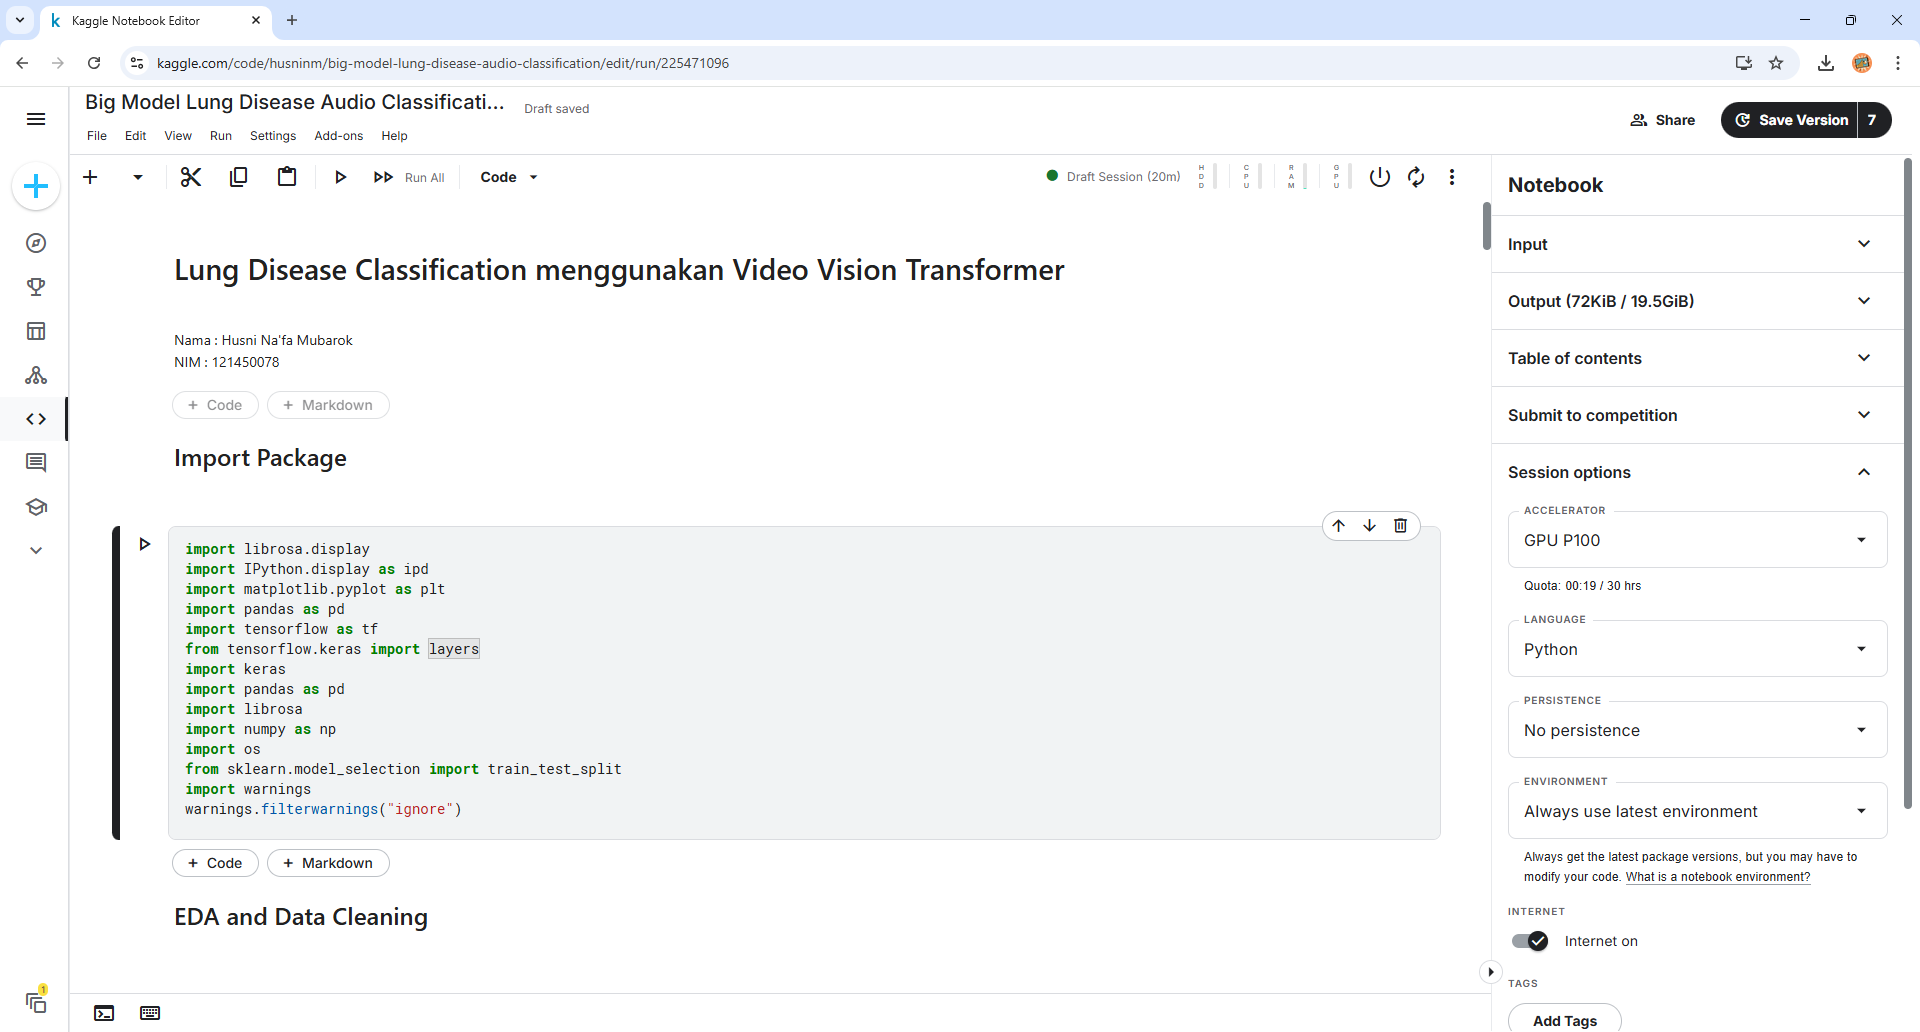
\includegraphics[width=1\linewidth]{gambar/Screenshot 2025-03-10 103758.png}
    \caption{\textit{Kaggle Workspace}}
    \label{fig:kaggle_workspace}
\end{figure}
\subsection{Import Package/Library yang digunakan}
\begin{table}[H]
    \centering
    \caption{Daftar Library Python dan Deskripsinya}
    \begin{tabular}{l p{8cm}}
        \hline
        \textbf{Library} & \textbf{Deskripsi} \\ \hline
        \texttt{librosa} & Digunakan untuk analisis dan pemrosesan audio, seperti ekstraksi fitur suara. \\
        \texttt{librosa.display} & Modul dari \texttt{librosa} untuk menampilkan dan memvisualisasikan data audio. \\
        \texttt{IPython.display} & Menyediakan fungsi untuk menampilkan media interaktif, seperti audio dan video di notebook Jupyter. \\
        \texttt{matplotlib.pyplot} & Digunakan untuk membuat visualisasi data, termasuk grafik dan diagram. \\
        \texttt{pandas} & Library untuk manipulasi dan analisis data dalam bentuk tabel (DataFrame). \\
        \texttt{tensorflow} & Framework untuk machine learning dan deep learning. \\
        \texttt{tensorflow.keras.layers} & Modul dari Keras dalam TensorFlow untuk membangun arsitektur jaringan saraf. \\
        \texttt{keras} & High-level API untuk membangun dan melatih model deep learning. \\
        \texttt{numpy} & Digunakan untuk komputasi numerik dan operasi array multidimensi. \\
        \texttt{os} & Modul standar Python untuk berinteraksi dengan sistem file dan direktori. \\
        %\texttt{sklearn.model_selection} & Modul dari \texttt{scikit-learn} yang digunakan untuk membagi dataset menjadi data latih dan uji. \\
        \texttt{warnings} & Modul untuk menangani dan menyembunyikan peringatan di Python. \\ \hline
    \end{tabular}
    \label{tab:library_python}
\end{table}

\section{\textit{Exploratory data analysis} dan \textit{Data Cleaning}}

\section{Pembagian Data \textit{(Data Splitting)}}
Data dibagi dengan perbandingan 80:20

\section{Pembuatan Pipeline \textit{Data Processing}}

\subsection{\textit{Audio Processing}}
Data suara diekstrak menggunakan ekstraksi fitur MFCC.
% \begin{table}[H]
% \centering
% \caption{Parameter kelulusan tugas akhir}
% \begin{tabular}{ clc }
% \hline
% \textbf{No.} & \textbf{Parameter } & \textbf{Nilai} \\
% \hline
% 1. & Penulisan & A \\
% 2. & Penulisan & A \\
% \hline
% \end{tabular}
% \label{table:nilai}
% \end{table}

\subsection{Feature Processing}
Berikut algoritma pemrosesan riwayat pasien \ref{algo:feature_process}


\subsection{Data Generator}
\begin{algorithm}[H]
\caption{PipeLine Model}
\begin{algorithmic}[1]

\Function{DataGenerator}{$data$}
    \ForAll{$row \in data$}
        \State $(mfcc, features, label) \gets \Call{ProcessRow}{row}$
        \State \Yield $(mfcc, features, label)$
    \EndFor
\EndFunction

\Function{CreateDataset}{$data, batch\_size$}
    \State Define dataset signature
    \State Create dataset using \Call{DataGenerator}{$data$}
    \State Batch, shuffle, and prefetch dataset
    \State \Return Dataset
\EndFunction

\Function{SplitData}{$data, test\_size, random\_state$}
    \State Split dataset into train and validation sets
    \State \Return $(train\_data, valid\_data)$
\EndFunction

\State $(train\_data, valid\_data) \gets \Call{SplitData}{data, 0.2, 25}$
\State $train\_dataset \gets \Call{CreateDataset}{train\_data, BATCH\_SIZE}$
\State $valid\_dataset \gets \Call{CreateDataset}{valid\_data, BATCH\_SIZE}$

\end{algorithmic}
\end{algorithm}

% \begin{equation}
%     x+2 = 159
% \end{equation}
% Bla bla bla bla

% %Berikut adalah contoh gambar yang dicetak secara horizontal
% \begin{landscape}
%    \begin{figure}[t]
%         \centering
%         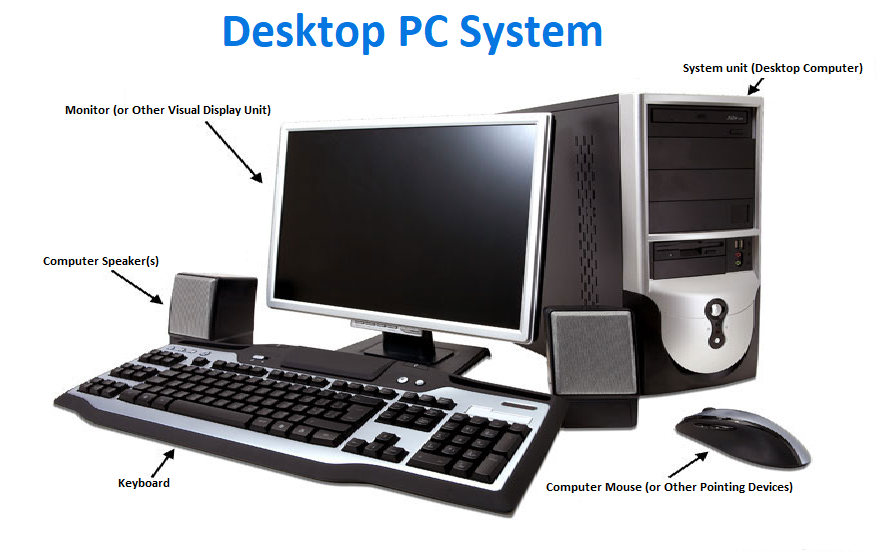
\includegraphics[width=18cm, height=12cm]{gambar/contoh-gambar-miring.png}
%          \caption{Contoh Gambar Komputer}
%         \label{fig:komputer}
%     \end{figure}
% \end{landscape}

\section{Pelatihan Model}
\subsection{Data Pelatihan dan Batching}
\subsection{Optimizer dan Regularisasi}
\subsection{Variasi Model}
\begin{table}[H]
    \centering
    \caption{Variasi parameter untuk model Transformer Small dan Big}
    \begin{tabular}{l|cccccccc|cc}
        \hline
        \textbf{Model} & $N$ & $d_\text{model}$ & $d_\text{ff}$ & $h$ & $d_k$ & $d_v$ & $P_\text{drop}$ & $\epsilon_\text{ls}$ & \textbf{Accuracy} & \textbf{Precision} \\

    \hline\rule{0pt}{2.0ex}
    \multirow{3}{*}{Small}
    & 6 & 32 & & 8 & 512 & 512 & & & 5.29 & 24.9  \\
    & & 64 & & & 128 & 128 & & & 5.00 & 25.5  \\
    & & 128 & & 16 & 32 & 32 & & & 4.91 & 25.8  \\
    \hline\rule{0pt}{2.0ex}
    \multirow{2}{*}{Big}
    & 12 & 64 & & & 16 & & & & 5.16 & 25.1 \\
    & & 128 & & & 32 & & & & 5.01 & 25.4 \\
    \hline
    \end{tabular}
    \label{tab:Variasi_Model}
\end{table}

\subsection{Perbandingan Positional Embedding dengan Trainable Embedding}
\begin{table}[H]
    \centering
    \caption{Perbandingan hasil antara Positional Embedding dan Trainable Embedding.}
    \begin{tabular}{lcc}
        \hline
        \textbf{Metric} & \textbf{Positional Embedding} & \textbf{Trainable Embedding} \\
        \hline
        Accuracy        & 85\%                          & 88\%                         \\
        Precision       & 83\%                          & 86\%                         \\
        Recall          & 82\%                          & 89\%                         \\
        F1-Score        & 82.5\%                        & 87\%                         \\
        \hline
    \end{tabular}
    \label{tab:embedding_comparison}
\end{table}
\section{Evaluasi Model}
\subsection{Akurasi dan Loss Pelatihan}

\subsection{Confussion Matrix}

\subsection{Kurva AUC-ROC}

\subsection{Prediksi Data baru}